% Auto-generated from experiment results. Do not edit manually.
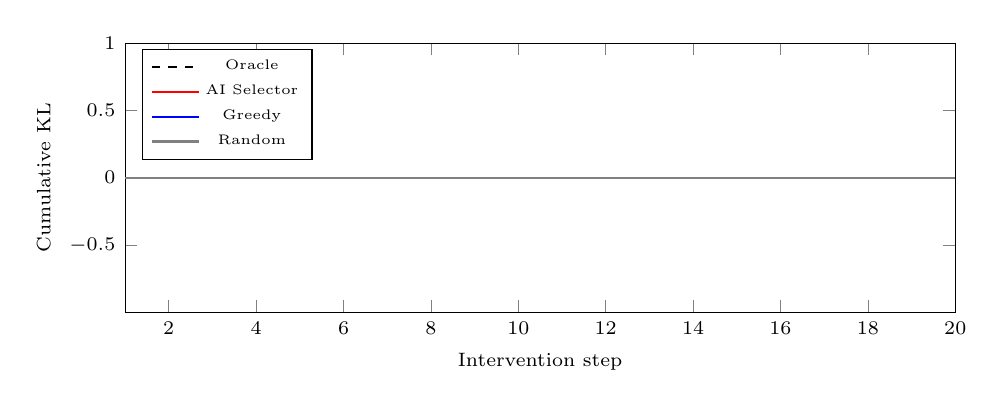
\begin{tikzpicture}
\begin{axis}[
    width=\columnwidth,
    height=5cm,
    xlabel={Intervention step},
    ylabel={Cumulative KL},
    x label style={font=\scriptsize},
    y label style={font=\scriptsize},
    tick label style={font=\scriptsize},
    legend style={
        font=\tiny,
        at={(0.02,0.98)},
        anchor=north west
    },
    xmin=1, xmax=20,
]

\addplot[black, dashed, thick] coordinates { (1,0.000000) (2,0.000000) (3,0.000000) (4,0.000000) (5,0.000000) (6,0.000000) (7,0.000000) (8,0.000000) (9,0.000000) (10,0.000000) (11,0.000000) (12,0.000000) (13,0.000000) (14,0.000000) (15,0.000000) (16,0.000000) (17,0.000000) (18,0.000000) (19,0.000000) (20,0.000000) };
\addplot[red, thick] coordinates { (1,0.000000) (2,0.000000) (3,0.000000) (4,0.000000) (5,0.000000) (6,0.000000) (7,0.000000) (8,0.000000) (9,0.000000) (10,0.000000) (11,0.000000) (12,0.000000) (13,0.000000) (14,0.000000) (15,0.000000) (16,0.000000) (17,0.000000) (18,0.000000) (19,0.000000) (20,0.000000) };
\addplot[blue, thick] coordinates { (1,0.000000) (2,0.000000) (3,0.000000) (4,0.000000) (5,0.000000) (6,0.000000) (7,0.000000) (8,0.000000) (9,0.000000) (10,0.000000) (11,0.000000) (12,0.000000) (13,0.000000) (14,0.000000) (15,0.000000) (16,0.000000) (17,0.000000) (18,0.000000) (19,0.000000) (20,0.000000) };
\addplot[gray, thick] coordinates { (1,0.000000) (2,0.000000) (3,0.000000) (4,0.000000) (5,0.000000) (6,0.000000) (7,0.000000) (8,0.000000) (9,0.000000) (10,0.000000) (11,0.000000) (12,0.000000) (13,0.000000) (14,0.000000) (15,0.000000) (16,0.000000) (17,0.000000) (18,0.000000) (19,0.000000) (20,0.000000) };

\legend{Oracle, AI Selector, Greedy, Random}

\end{axis}
\end{tikzpicture}
